\documentclass[12pt]{article}


\usepackage[utf8]{inputenc}
\usepackage[a4paper,top=3cm,bottom=2cm,left=3cm,right=3cm,marginparwidth=1.75cm]{geometry}
\usepackage[nodayofweek]{datetime}
\usepackage{tabularx}
\usepackage[small]{titlesec}
\usepackage{graphicx}
\usepackage{tabularx}

\newcolumntype{L}[1]{>{\raggedright\arraybackslash}p{#1}}
\newcolumntype{C}[1]{>{\centering\arraybackslash}p{#1}}
\newcolumntype{R}[1]{>{\raggedleft\arraybackslash}p{#1}}

\begin{document}

\begin{titlepage}
    \begin{center}
        \huge{\bfseries  Tribhuvan University}\\
        \Large{Institute of Engineering}\\
        \huge{ \bfseries  Pulchowk Campus}\\[3.2cm]


        \textsc{\Large Big Data Technologies}\\[-0.5cm]
        \line(1,0){400}\\
        \huge{\bfseries No SQL database architectures}\\
        \large{Hbase, Casasndra, MongoDB}
        \line(1,0){400}\\


        \textsc{\Large Submitted by:}\\
        \Large Bishal Katuwal\\ \large 075BCT028\\    [0.85cm]

        \textsc{\Large Submitted to:}\\\
        \large Department of Electronics and Computer Engineering\\Pulchowk Campus\\    [0.85cm]
        
        \textsc{\Large Submitted on:}\\
        \today
        
    \end{center}
\end{titlepage}
\pagebreak
% ===============================================================
\section{Hbase}
\subsection{Introduction}
HBase is a distributed NoSQL database that runs on top of the Hadoop Distributed File System (HDFS). It is a column-oriented database management system that is designed to handle large amounts of structured data and provide real-time read/write access to that data. It is highly scalable. The architecture of HBase consists of three main components. They are : 
\begin{itemize}
    \item ZooKeeper
    \item RegionServers
    \item HMaster
\end{itemize}
 
\subsection{Architecture}
The architecture of HBase consists of the following components: 
\begin{itemize}
    \item {\bfseries Zookeeper}: \\
    HBase uses Apache ZooKeeper to manage the distributed coordination of the HBase cluster. ZooKeeper ensures that all the nodes in the cluster are synchronized and up to date. It keeps track of the state of the cluster and helps in leader election.
    \item {\bfseries Region Server}: \\
    HBase is designed to scale horizontally by distributing data across multiple nodes in a cluster. Each node is called a Region Server and is responsible for managing a set of regions, which are portions of the overall dataset. They are the nodes that store the actual data. Each regionServer manages one or more regions of the table. A region is a contiguous range of rows in the table.
    \item {\bfseries Master Server}:\\
    Master Server is responsible for monitoring and managing the Region Servers in the cluster. It performs tasks such as load balancing, failover,and region assignment. It is responsible for managing the metadata of the tables and the RegionServers. It handles operations like table creation, deletion, and splitting.
    \item {\bfseries HDFS}:\\
    HBase stores its data in HDFS, which provides a fault-tolerant and scalable distributed file system for storing large datasets.
    \item {\bfseries HBase client}:\\
    Applications that need to access data stored in HBase interact with the database through the HBase client API. The HBase client communicates with the HBase cluster to retrieve and store data.
\end{itemize}

The data in HBase is organized into tables, which are divided into rows and columns. Each row in a table has a unique row key that identifies it, and each column in a row is identified by a column family and a column qualifier. HBase supports automatic sharding of tables, which means that as the size of the dataset grows, it can be split across multiple Region Servers for improved performance and scalability.

To understand the architecture of Hbase, following concepts should be understood.
\begin{itemize}
    \item {\bfseries Write-Ahead Log}
    The Write-Ahead Log is a file that HBase uses to ensure data durability. Whenever a write operation occurs, HBase writes the data to the WAL first, before the data is written to the MemStore. The WAL is stored on disk and provides a mechanism for recovering data in the event of a node failure or crash. When a RegionServer starts up, it reads the contents of the WAL and applies any outstanding write operations to the MemStore. This ensures that data is not lost due to a node failure or crash.
    \item {\bfseries MemStore}
    The MemStore is an in-memory buffer that holds the most recent writes to a region. Whenever a write operation occurs, HBase writes the data to the MemStore first. The MemStore is a write-intensive cache, optimized for high-throughput write operations. When the MemStore is full, its contents are flushed to disk, creating a new HFile on the local file system. The HFiles are immutable and provide efficient random read access, making them optimized for read-intensive workloads.
\end{itemize}
\begin{figure}[h!]
    \centering
    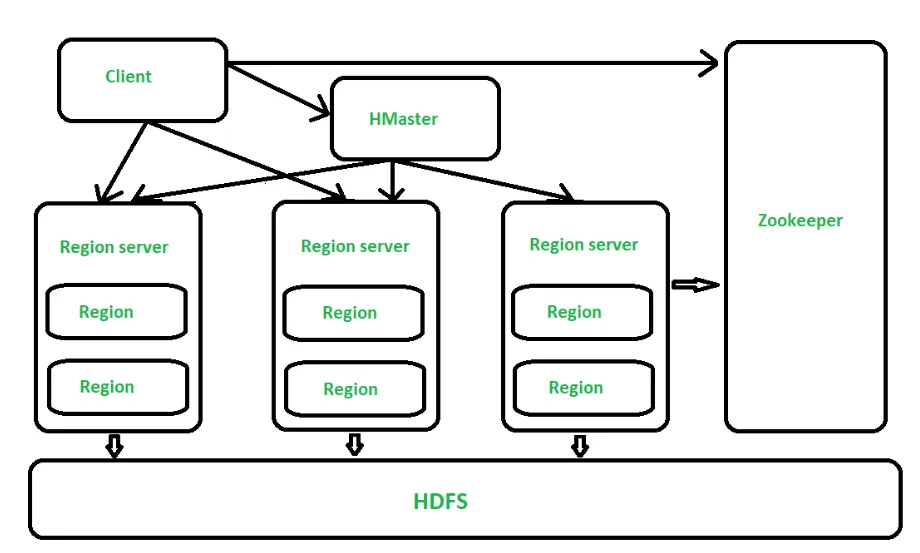
\includegraphics[scale = 0.5]{images/Hbase.png}
    \caption{Hbase architecture}
\end{figure}
\subsection{Working of HBase}
\subsubsection{Write}
When a client wants to write data, it sends a write request to the RegionServer responsible for the region that contains the data. The RegionServer
validates the write request and, if the request is valid, writes the data to the write-ahead log (WAL) on the local disk for durability. The RegionServer then applies the write to the MemStore. When the MemStore is full, its contents are flushed to disk, creating a new HFile on the local file system. Once the data is written to the local disk, the RegionServer replicates the data to other RegionServers in the cluster.
\subsubsection{Read}
When a client wants to read data, it sends a read request to the RegionServer responsible for the region that contains the data. The RegionServer reads the data from the HFiles on its local file system or from the MemStore if the data has not yet been flushed to disk. If the requested data is not in the RegionServer's local cache, it retrieves the data from other RegionServers in the cluster through a process called data locality. The RegionServer returns the data to the client.
\subsection{Conclusion}
Overall, HBase uses a distributed architecture where data is partitioned into regions and stored on multiple RegionServers. This architecture provides high availability, fault tolerance, and scalability. HBase also provides efficient data locality to minimize the network traffic required for read operations.
\pagebreak
\section{Casasndra}
\subsection{Introduction}
Cassandra is a distributed, non-relational database management system designed to handle large amounts of structured and unstructured data across multiple data centers. It is based on a peer-to-peer architecture that allows nodes to communicate with each other without a central coordinator. It is a distributed database that is designed to handle large amounts of data across multiple commodity servers. It has a masterless architecture, where all nodes are equal and communicate with each other.
The architecture of Cassandra consists of:
\begin{itemize}
    \item Node
    \item Datacenter
    \item Cluster
    \item Coordinator
\end{itemize} 
 
\subsection{Architecture}
The architecture of Cassandra consists of following components:
\begin{itemize}
    \item {\bfseries Node : \\}
    A node in Cassandra is a physical or virtual machine that runs the Cassandra software. It is the basic building block of the cluster. Each node is responsible for storing a portion of the data, and can communicate with other nodes in the cluster to retrieve or update data.
    \item {\bfseries Datacenter :\\}
    A datacenter is a logical grouping of nodes that are geographically close to each other and are configured to be highly available. Each datacenter in a cluster can be configured with its own replication factor, consistency level,
    and other settings.
    \item {\bfseries Cluster : \\}
    A cluster in Cassandra is a collection of one or more datacenters that work together to provide fault-tolerant and scalable storage for data.
    \item {\bfseries Coordinator : \\}
    It is responsible for handling client requests and routing them to the appropriate nodes.
\end{itemize}

The architecture of Cassandra also involves: 
\begin{itemize}
    \item {\bfseries Commit Log : \\}
    Cassandra uses a commit log to ensure data durability. When data is written to Cassandra, it is first written to the commit log on disk before it is written to the in-memory data structures.
    \item{\bfseries Memtable : \\}
    The memtable is an in-memory data structure that stores data that has been recently written to Cassandra. Data in the memtable is periodically flushed to disk to ensure data durability.
    \item {\bfseries SSTable : \\}
    An SSTable (Sorted String Table) is a disk-based data structure that stores data that has been flushed from the memtable. SSTables are immutable, meaning that once they are written to disk, they cannot be modified.
    \item {\bfseries Partitioner : \\}
    Cassandra uses a partitioner to distribute data evenly across nodes in the cluster. The partitioner is responsible for generating a token for each row in a table, which determines which node the data should be stored on.
    \item{\bfseries Replication : \\}
    Cassandra uses replication to ensure data availability and fault tolerance. Each datacenter in the cluster can be configured with its own replication factor, which determines how many copies of each piece of data should be stored in the datacenter.
\end{itemize}
\begin{figure}[h!]
    \centering
    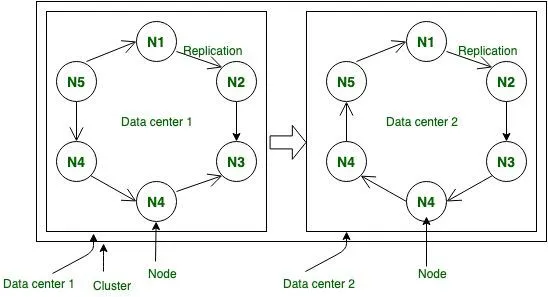
\includegraphics[scale = 0.7]{images/Cassandra.png}
    \caption{Cassandra Architecture}
\end{figure}
\subsection{Working of Cassandra}
  \subsubsection{Write}
  When a client wants to write data, it sends a write request to one of the nodes in the cluster, called a coordinator node. The coordinator node determines the nodes responsible for storing the data based on the hash value of the partition key of the data. The coordinator node then sends a write request to all the replica nodes that are responsible for storing the data. The replica nodes acknowledge the write operation once the data has been successfully written to their local disk. Once enough replicas has acknowledged the write, the coordinator node sends an acknowledgment to the client, indicating that the write was successful.
  \subsubsection{Read}
  When a client wants to read data, it sends a read request to one of the nodes in the cluster, called a coordinator node. The coordinator node determines the nodes responsible for storing the data based on the hash value of the partition key of the data. The coordinator node then sends a read request to all the replica nodes that are responsible for storing the data. The replica nodes return the data to the coordinator node. The coordinator node waits for the required number of replicas to respond based on the consistency level specified by the client. Once the required number of replicas has responded, the coordinator node returns the data to the client.
\subsection{Conclusion}
Overall, Cassandra uses a decentralized architecture and consistent hashing to distribute data across multiple nodes in the cluster. Each node acts as a
coordinator for some data and as a replica for other data. This architecture provides high availability, fault tolerance, and scalability.
  \pagebreak
\section{MongoDB}
\subsection{Introduction}
MongoDB is a NoSQL document-oriented database that is designed to store and manage unstructured data. Its architecture is based on a distributed cluster
model, and it supports horizontal scaling through the use of sharding. It stores data in collections and documents. It is designed to be highly scalable and flexible. The architecture
of MongoDB consists of the following components:
\begin{itemize}
    \item Replica Set
    \item Shard
    \item Config Servers
    \item Router
\end{itemize}
  
\subsection{Architecture}
\begin{itemize}
    \item {\bfseries Replica Set : \\}
    A replica set is a group of MongoDB servers that maintains the same data set. They work together to provide redundancy and high availability. A replica set typically consists of three or more servers, with one server designated as the primary and the others as secondary servers.
    \item {\bfseries Shard : \\}
    A shard is a horizontal partition of data across multiple servers. Each shard is responsible for storing a subset of the data.
    \item{\bfseries Config Servers : \\}
    Config Servers are responsible for maintaining the metadata of the cluster, such as the location of the shards and the mapping of data to shards.
    \item {\bfseries Router : \\}
    It is responsible for routing client requests to the appropriate shards and maintaining a connection to the config servers.
\end{itemize}
To understand the architecture of MongoDB following concepts should be understood.
\begin{itemize}
    \item {\bfseries MongoDB Cluster : \\}
    A MongoDB cluster consists of one or more MongoDB servers that are deployed on different physical or virtual machines. The servers in the cluster communicate with each other to manage data and provide high availability and fault tolerance.
    \item{\bfseries Sharding : \\}
    Sharding is the process of partitioning a large dataset across multiple servers. In MongoDB, sharding is used to horizontally scale data across multiple servers in a cluster. Sharding is achieved by splitting a dataset into smaller chunks called shards and distributing them across multiple servers.
    \item{\bfseries Documents : \\}
    MongoDB stores data in the form of documents, which are JSON-like objects that contain data and metadata. Documents are grouped into collections, which are similar to tables in a relational database.
    \item{\bfseries Indexes : \\}
    MongoDB supports the creation of indexes to improve the performance of data retrieval operations. Indexes are created on specific fields in a collection and are used to quickly locate data in the collection.
    \item{\bfseries WiredTiger Storage Engine: \\}
    MongoDB uses the WiredTiger storage engine as the default storage engine. WiredTiger uses a document-level concurrency control approach to provide high concurrency and performance.
    \item{\bfseries Drivers : \\}
    MongoDB provides drivers for many programming languages, which allow applications to interact with the MongoDB database.
\end{itemize}
\begin{figure}[h!]
    \centering
    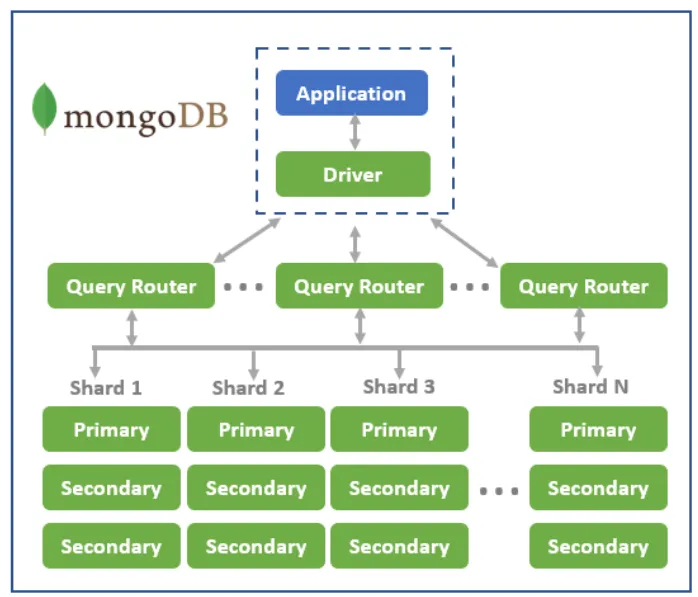
\includegraphics[scale = 0.6]{images/MongoDB.png}
    \caption{Architecture of MongoDB}
\end{figure}
\subsection{Working of MongoDB}
\subsubsection{Write}
When a client wants to write data, it sends a write request to the primary node in the replica set. The primary node validates the write request and, if the request is valid, writes the data to its local storage engine. Once the data is written to the primary node, the primary node replicates the data to the secondary nodes in the replica set. Once enough nodes has acknowledged the write, the primary node sends an acknowledgment to the client, indicating that the write was successful. 
\subsubsection{Read}
When a client wants to read data, it sends a read request to any node in the replica set. If the client specifies a read preference, the request will be sent to a node that satisfies the preference. If the requested data is not in the node's memory, the node reads the data from the local storage engine or, if the node is a secondary node, from the primary node. The node returns the data to
the client.
\subsection{Conclusion}
Overall, MongoDB uses a replica set architecture to provide high availability and fault tolerance. The primary node handles all write operations and
replicates data to secondary nodes, while any node in the replica set can handle read operations. MongoDB also supports sharding, which allows data to be distributed across multiple nodes in a cluster, providing scalability.
\pagebreak
\section{Conclusion}
In conclusion, HBase, Cassandra, and MongoDB are NoSQL databases that have different architectures and usage. HBase is column-oriented and built on Hadoop, Cassandra is a masterless architecture, and MongoDB is document-oriented. Understanding the architecture of each database can help in selecting the appropriate one for given use case. It is important to note that each database has its strengths and weaknesses. HBase is ideal for read-heavy workloads, Cassandra is designed for write-heavy workloads, and MongoDB is great for
flexibility and ease of use. When selecting a database, it is important to consider specific use case and the requirements of given application. NoSQL databases are becoming increasingly popular due to them being designed to be highly scalable and flexible, making them ideal for modern use cases.
\end{document}